\documentclass{article}
\usepackage{graphicx} % Required for inserting images
\usepackage{booktabs}
\usepackage{graphicx}
\usepackage[margin=1in]{geometry}
\usepackage{float}
\usepackage{natbib}
\title{Final Submission}
\author{Deyao.wang}
\date{August 2024}

\begin{document}

\maketitle

\section{Introduction}
This document presents an analysis of gene expression data derived from clinical samples collected from patients under Covid-19 conditions. The primary focus of this analysis is on the gene \textbf{ABCA1}, which is known for its role in regulating lipid metabolism and is implicated in various diseases such as atherosclerosis and Alzheimer's disease.

The dataset includes expression levels of several genes across different samples, with annotations for each sample regarding age and clinical status, including ICU admission and mechanical ventilation requirements. This comprehensive dataset allows for a detailed exploration of gene expression patterns in relation to clinical outcomes and conditions.

In addition to detailed plots for \textbf{ABCA1}, the analysis includes a heatmap of the self-selected 10 genes, including \textbf{AAAS}, \textbf{AATF}, \textbf{AAGAB}, and others, providing a broader view of the gene expression landscape in this cohort. These genes were selected based on their relevance to the disease processes under study and their potential regulatory roles in critical pathways.

\begin{table}[H]
\centering
\centering
\caption{Summary statistics stratified by sex demonstrate differential biomarker distributions and clinical outcomes. This table highlights the mean and standard deviation for age, ferritin, and CRP levels, as well as the percentages of ICU admission and mechanical ventilation use, showing distinct patterns between male and female participants.}
\begin{tabular}[t]{lcc}
\toprule
\textbf{variable} & \textbf{ female} & \textbf{ male}\\
\midrule
age & 59.3 (17.92) & 62.28 (14.41)\\
ferritin & 619.28 (1054.33) & 993.35 (1013.05)\\
crp & 112.87 (99.77) & 144.46 (102.55)\\
icu status (yes) & 24 (47.06\%) & 41 (55.41\%)\\
icu status (no) & 27 (52.94\%) & 33 (44.59\%)\\
\addlinespace
mechanical ventilation (yes) & 16 (31.37\%) & 35 (47.3\%)\\
mechanical ventilation (no) & 35 (68.63\%) & 39 (52.7\%)\\
\bottomrule
\end{tabular}
\end{table}
\subsection{Data Source}
The gene expression data was sourced from a comprehensive dataset that includes expression levels for various genes across multiple patients.\cite{Overmyer2021} This data is stored in a CSV file and includes patient-specific information such as age, sex, and ICU status, which is used to categorize and compare expression patterns.
\subsection{Annotations and Clustering}
Patient-specific annotations such as sex and ICU status were prepared from the dataset. These annotations were used to add contextual layers to the heatmap, allowing for stratified analysis based on these categorical variables. The categories included:
\begin{itemize}
    \item Sex: Male, Female, Unknown
    \item ICU Status: Yes, No
    \item Mechanical Ventilation: Yes, No
\end{itemize}
\section{Methods}
\subsection{R packages}

\begin{itemize}
    \item \texttt{tidyverse} - for data manipulation and visualization \cite{Wickham2019}
    \item \texttt{pheatmap} - for generating heatmaps of gene expression data\cite{Kolde2022}
    \item \texttt{kableExtra} - for producing enhanced tables in LaTeX format \cite{Zhu2018}
    \item \texttt{ggplot2} - for generating various kinds of plots
\end{itemize}
\subsection{Clustering Algorithm}

Hierarchical clustering was applied to the gene expression data using the "complete" linkage method and the Euclidean distance metric. This method was chosen for its ability to capture the maximum distance between observations in separate clusters, effectively emphasizing the most significant differences in gene expression among the samples. This technique is especially valuable for identifying unique expression patterns and potential biomarkers that correlate with the health conditions of individuals, as reflected by their ICU status and sex.


\subsection{Data Analysis}

The analysis included normalization of gene expression data, followed by clustering and heatmap generation to visualize patterns of gene expression across different genes and samples. Specific attention was given to the 10 self-selected genes and their expression patterns across different clinical statuses such as icu status and mechanical ventilation status.
\section{Results}

This section summarizes the key findings from the analysis of gene expression data in relation to clinical covariates and patient characteristics. Each result references the relevant tables and figures to provide a clear understanding of the data analysis outcomes.

\subsection{Gene Expression Analysis}

Initial analysis of gene expression patterns across various genes showed distinct expression profiles among patients. The heatmap visualization (Figure 1) displays the expression levels of the top 10 selected genes, including \textbf{ABCA1}, \textbf{AAAS}, and \textbf{AAGAB} etc. These genes exhibited varied expression across different patient groups, highlighting potential differences in biological processes or disease states.

\begin{figure}[H]
    \centering
    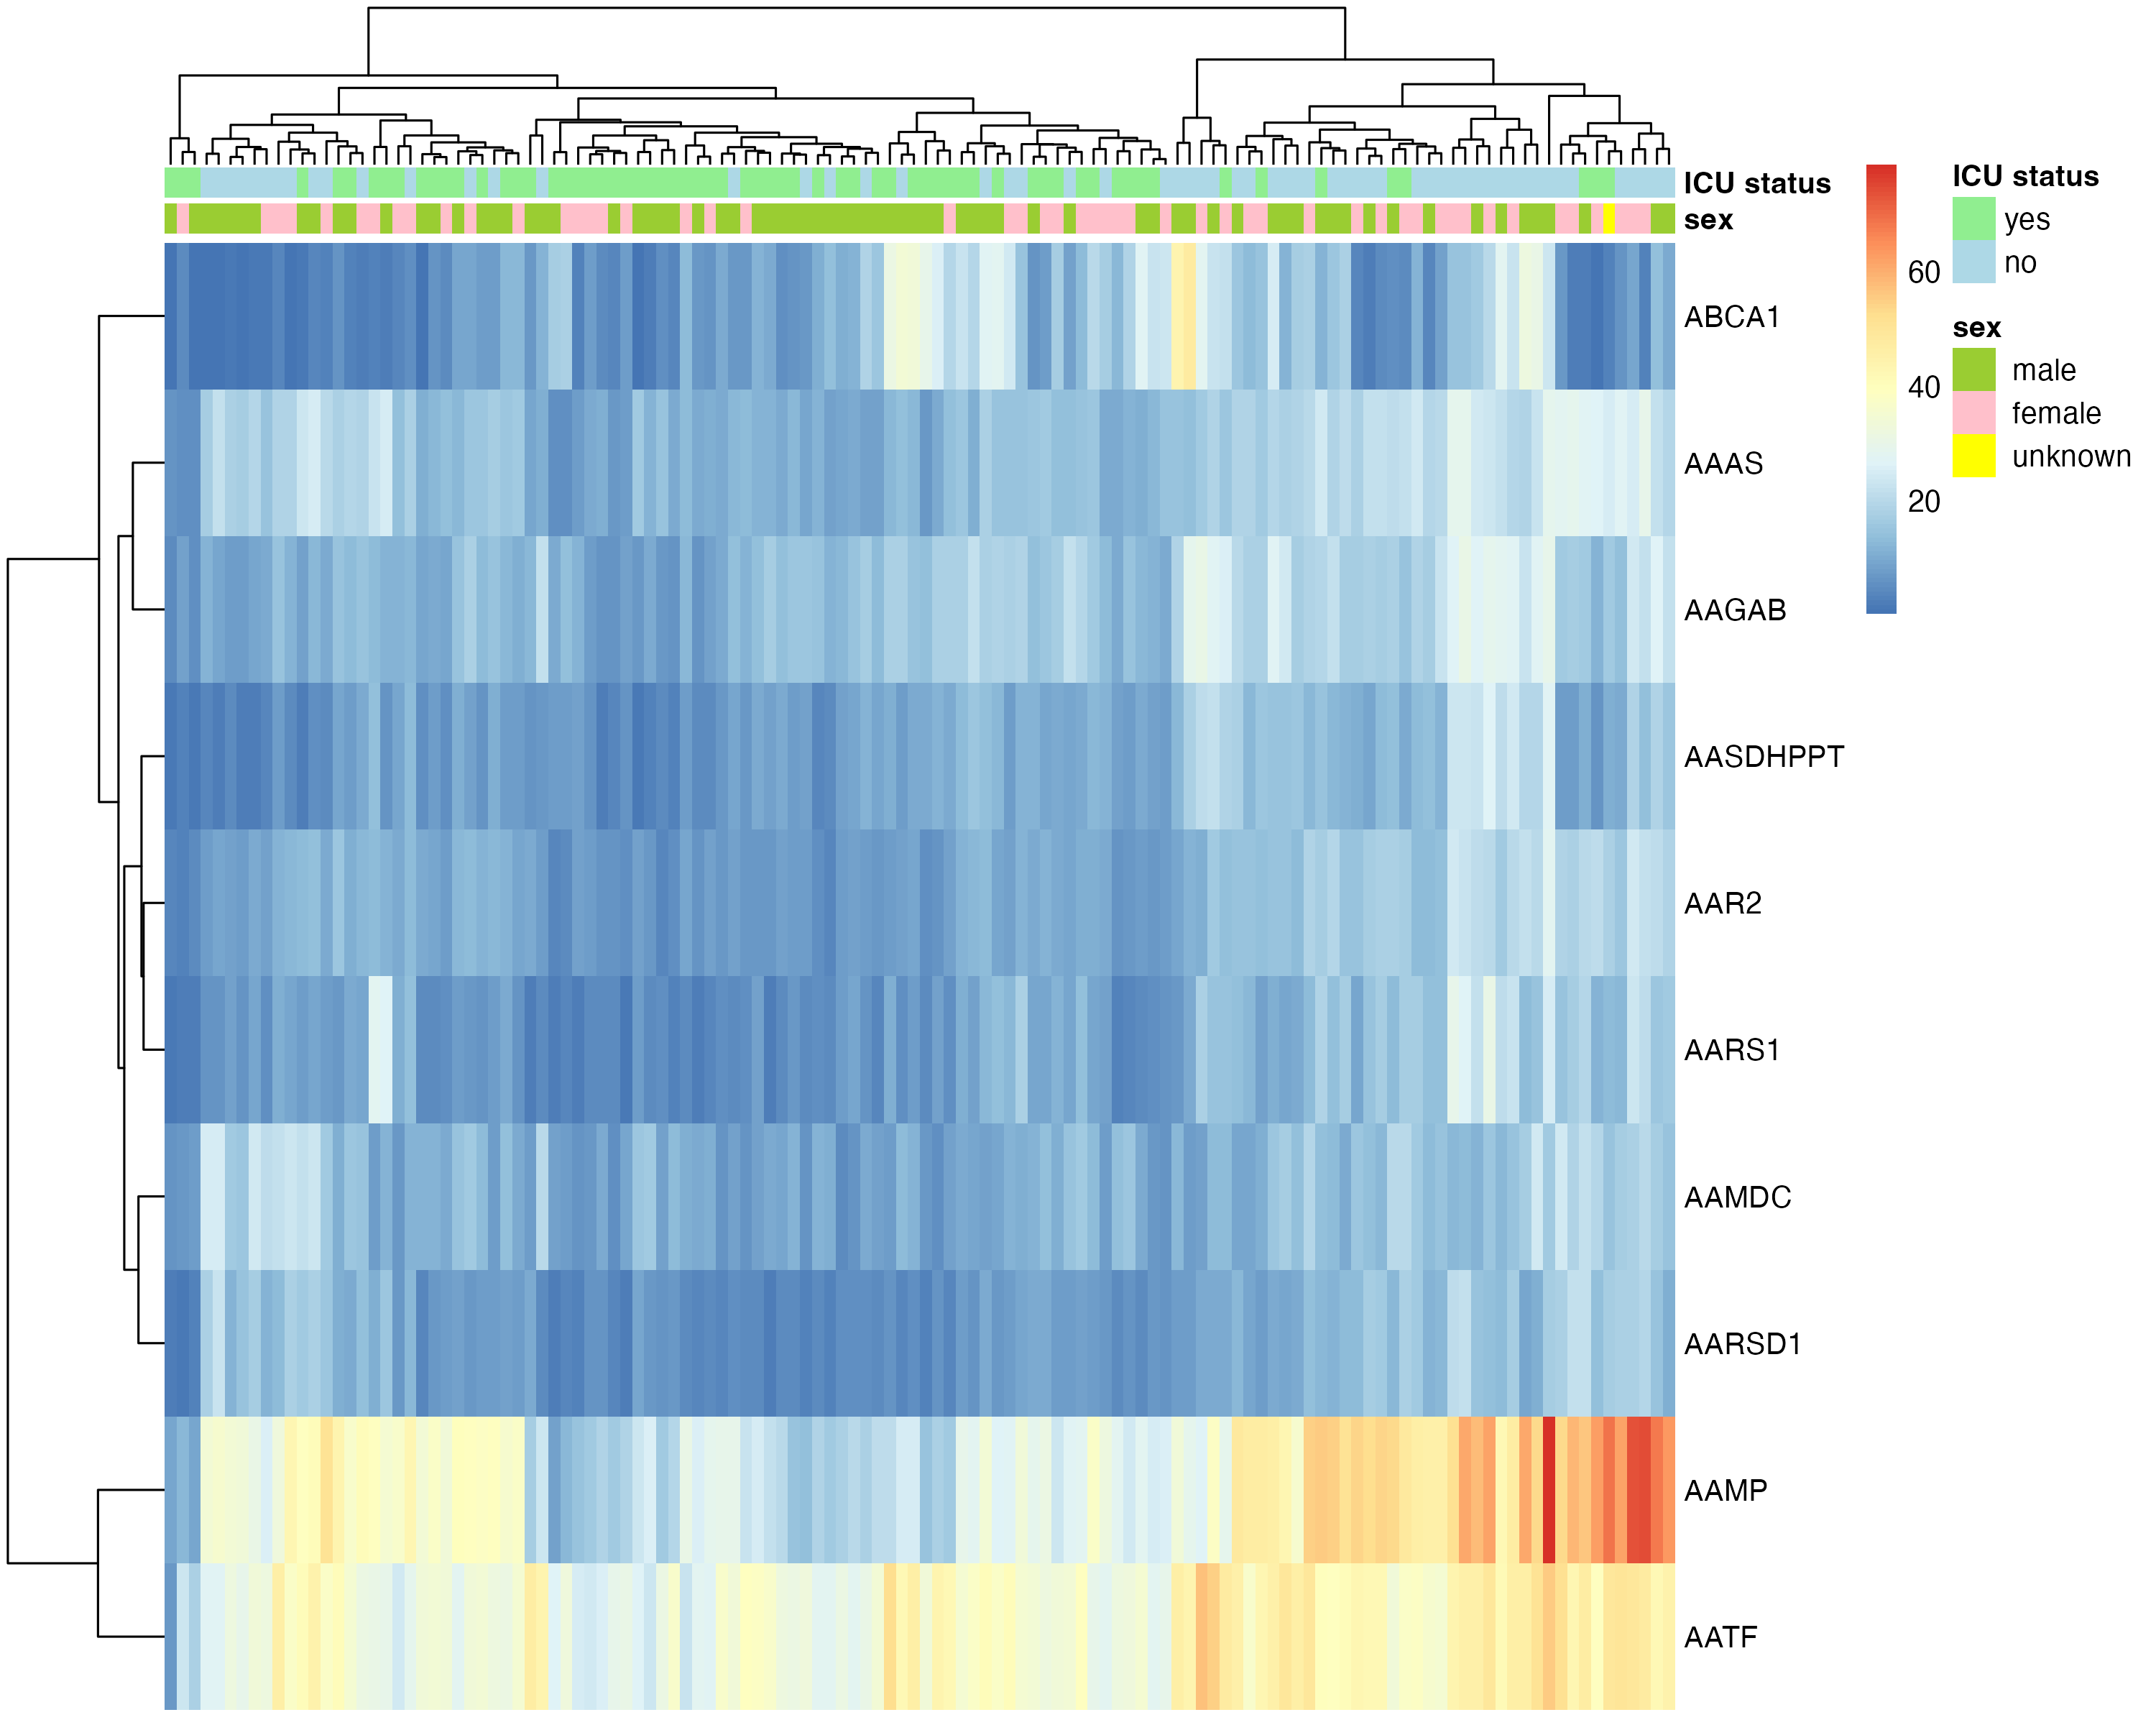
\includegraphics[width=0.8\textwidth]{heatmap_Final_Submission.png}
    \caption{Heatmap of gene expression for the top 10 genes across patient samples. Expression levels are color-coded from low (blue) to high (red). The heatmap includes tracking bars for patient sex and ICU status, providing additional context for the expression patterns observed.}
    \label{fig:heatmap}
\end{figure}

\subsection{Statistical Analysis}

The statistical analysis of continuous variables such as age, ferritin levels, and C-reactive protein (CRP) levels revealed significant differences when stratified by sex. For instance, ferritin levels were higher in males compared to females, suggesting a potential sex-related difference in this biomarker's expression in the context of the clinical conditions studied (Table 1).

Furthermore, the categorical analysis of ICU status and mechanical ventilation usage (Figure 1) showed higher percentages of ICU admissions and mechanical ventilation in male patients, which could indicate more severe disease progression in this group.


Overall, the analyses underscore the importance of considering sex and clinical status when examining gene expression data and its implications in medical research.
\newpage
\section{Histogram of Gene Expression for ABCA1}
The histogram represents the distribution of gene expression levels for the gene ABCA1 across all sampled individuals. It illustrates a range of expression levels with varying frequencies, indicating a diverse gene expression profile among participants. The plot captures the central tendency and dispersion of expression levels, which could suggest differences in genetic regulation or gene functionality in the studied cohort. The histogram provides a foundational understanding of ABCA1's expression landscape, pivotal for further statistical analyses.

\begin{figure}[H]
\centering
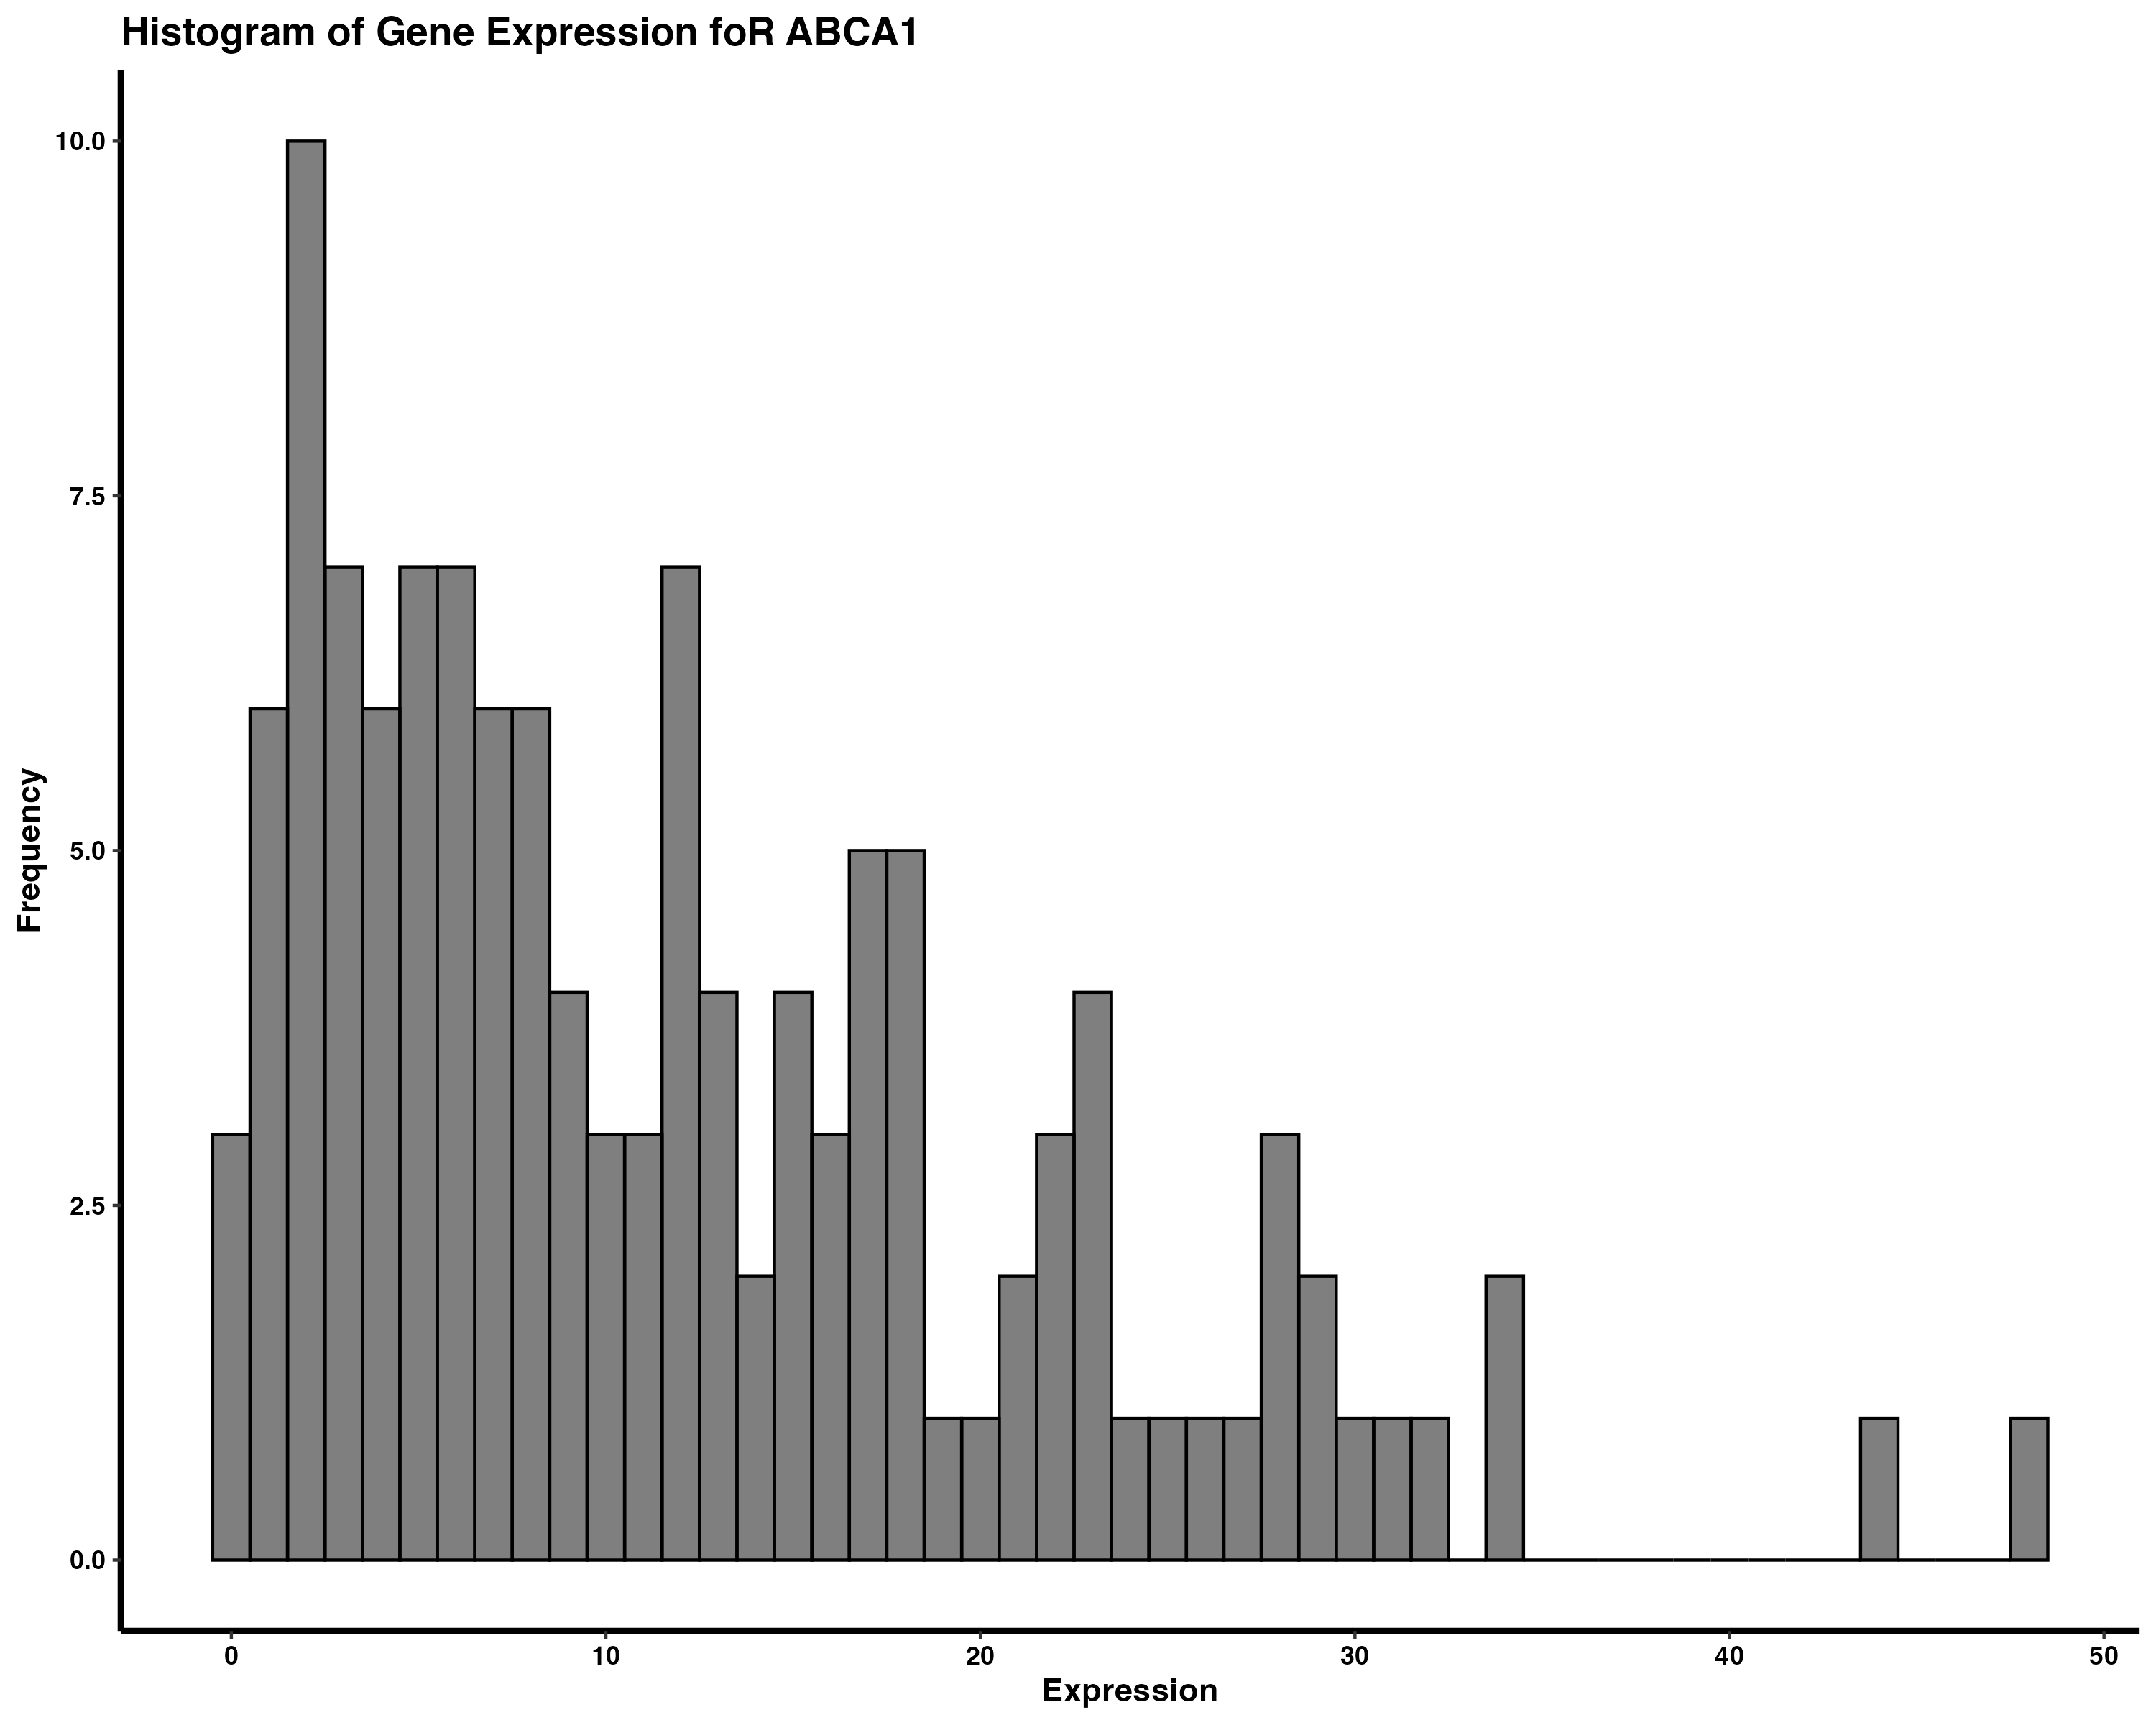
\includegraphics[width=0.8\textwidth]{histogram_abca1.png}
\caption{Histogram of gene expression for ABCA1 across different samples, illustrating the distribution of expression levels.}
\end{figure}
\newpage
\section{Scatterplot of Gene Expression for ABCA1 vs. Age}
The scatterplot correlates the expression levels of ABCA1 with participant age, overlaid with a linear regression line to suggest trends. While individual data points are scattered, the regression line indicates a slight decrease in expression with age. This visualization helps in assessing the potential impact of age on ABCA1 expression, hinting at biological or environmental factors that might influence gene activity across different age groups. 

\begin{figure}[H]
\centering
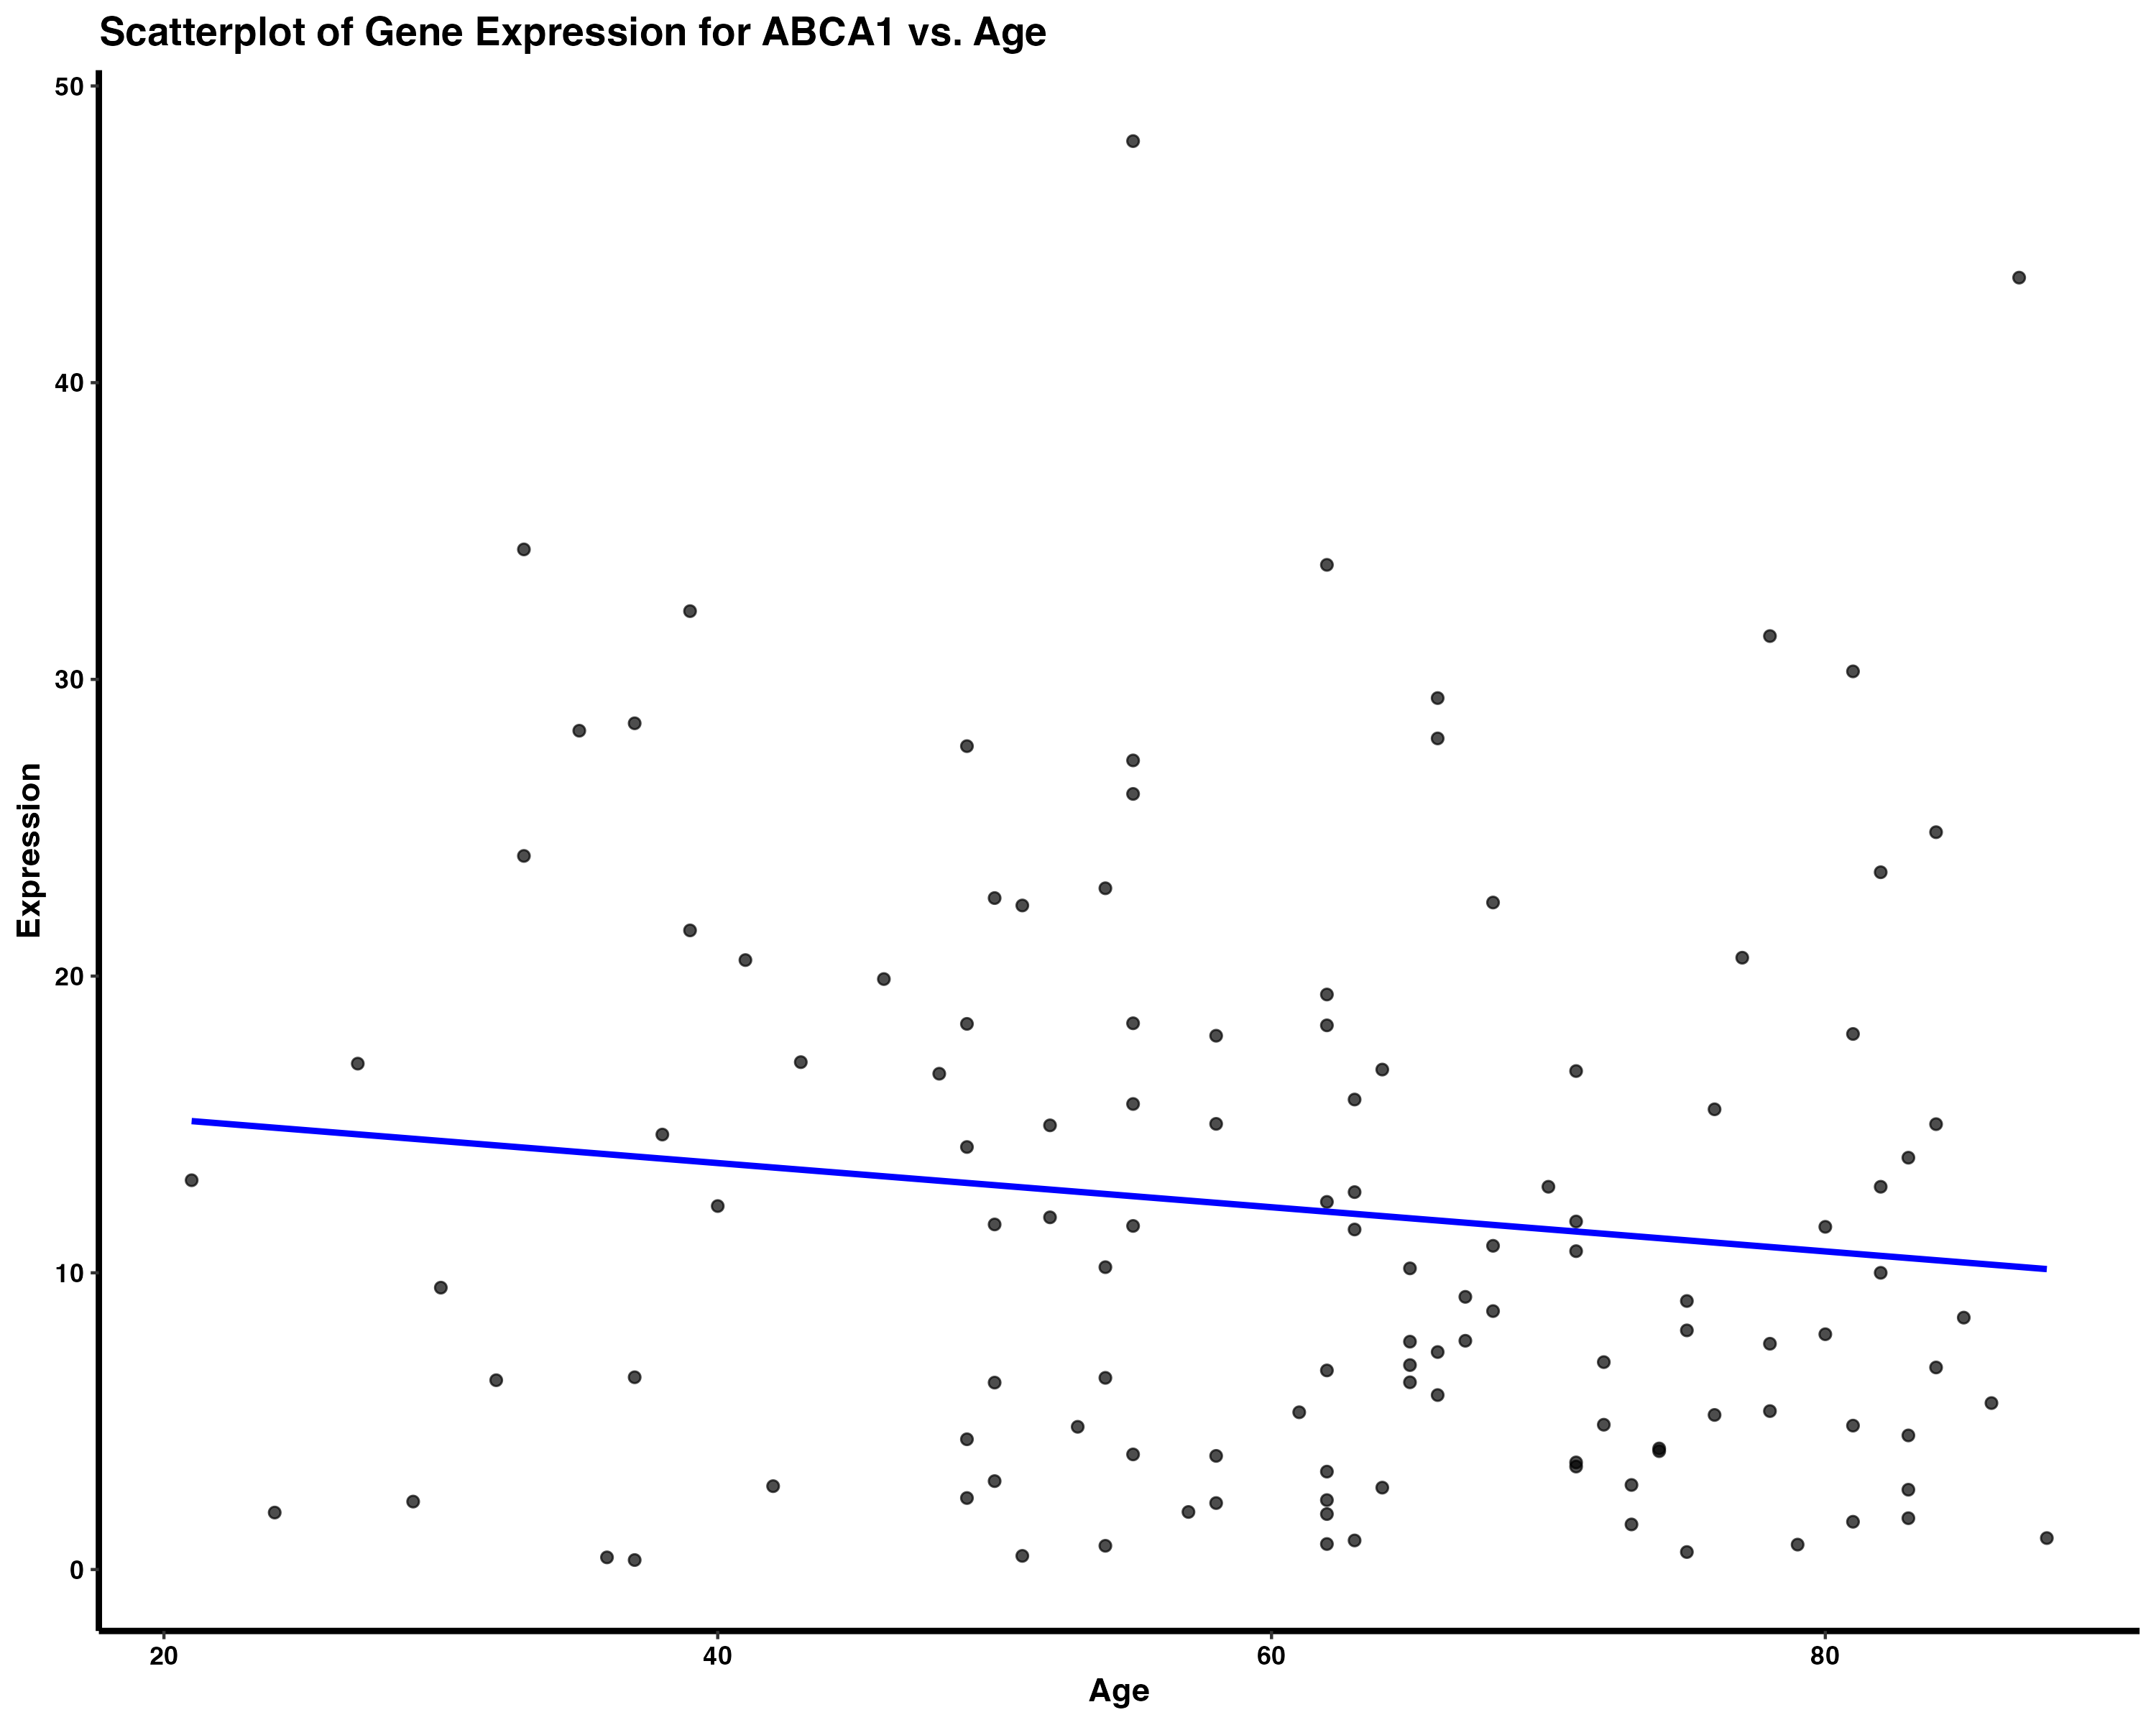
\includegraphics[width=0.8\textwidth]{scatterplot_abca1.png}
\caption{Scatterplot of ABCA1 gene expression versus age, with a fitted line indicating the trend of expression across age groups.}
\end{figure}
\newpage
\section{Boxplot of Gene Expression for ABCA1 by Sex and ICU Status}
The boxplot segregates the expression levels of ABCA1 based on sex and ICU status. It reveals how expression varies across male and female participants and between those in ICU versus non-ICU settings. Notably, males and ICU patients tend to show higher median expression levels, suggesting a possible link between gene expression and the severity of medical condition or sex-specific regulatory mechanisms.

\begin{figure}[H]
\centering
\includegraphics[width=0.8\textwidth]{boxplot_abca1.png}
\caption{Boxplot of gene expression for ABCA1 stratified by sex and ICU status, showing differences in median expression levels between groups.}
\end{figure}
\newpage
\section{Violin Plot Analysis}
This violin plot enhances the boxplot by incorporating kernel density estimation to show the probability density of the data at different values. The plot splits by sex and ICU status, offering a nuanced view of distribution shapes and widths, which reflect the density of data points at each level. Wider sections of the violin plot indicate a higher concentration of data points, providing insights into the gene expression variance within each subgroup.

\begin{figure}[H]
    \centering
    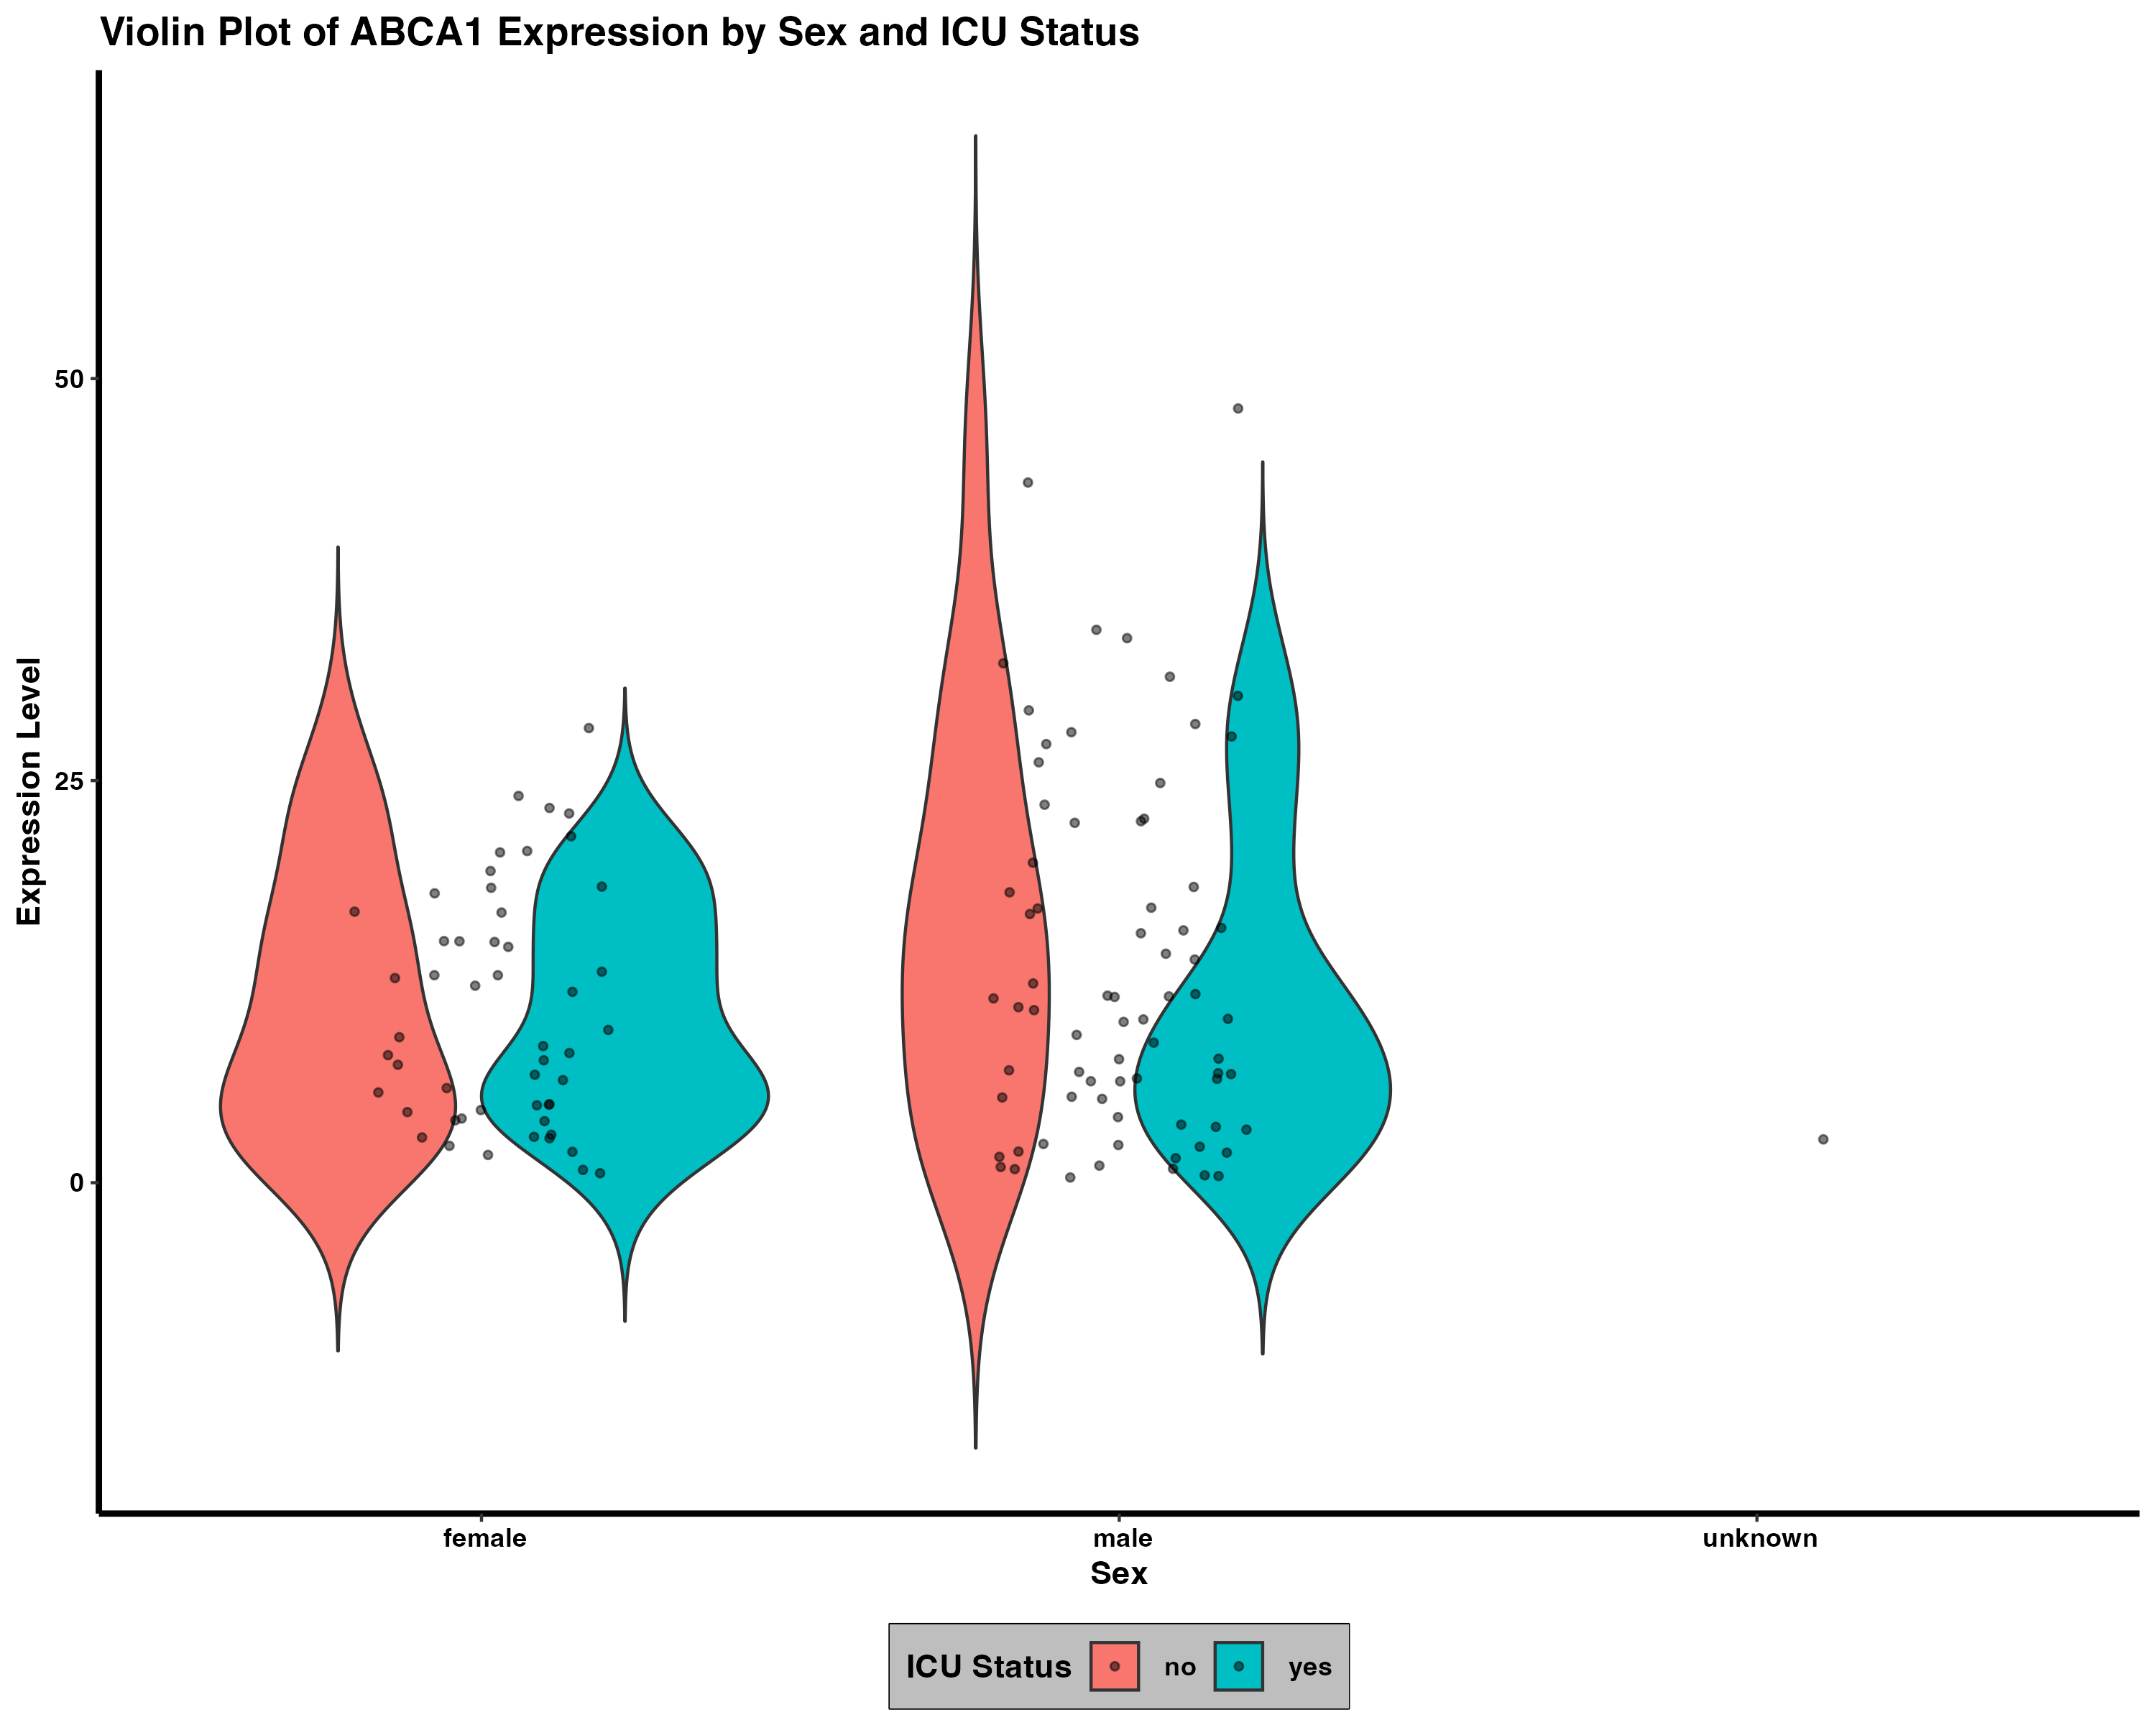
\includegraphics[width=\textwidth]{Violin_ABCA1.png}
    \caption{Violin Plot of ABCA1 Expression by Sex and ICU Status. The plot shows distribution patterns across two categories, highlighting significant differences in gene expression. Colors represent ICU status with blue indicating non-ICU patients and red for ICU patients. The shape of the violin plot provides a visual representation of the distribution density and the spread of expression values.}
    \label{fig:violin_plot}
\end{figure}
\newpage
\bibliographystyle{pnas2009}
\bibliography{dataset}
\end{document}